\documentclass[12pt,a4paper]{report}

\usepackage[utf8]{inputenc}
\usepackage[T1]{fontenc}
\usepackage[english]{babel}
\usepackage[top=1cm,bottom=2cm,left=1cm,right=1cm]{geometry}
%\usepackage{url}
%\usepackage{fancyhdr}
\usepackage{sectsty}
\usepackage{wrapfig}
\usepackage{titlesec}
\usepackage{setspace}
\usepackage{graphicx}
\usepackage{lmodern}
\usepackage{url}
\usepackage{amsmath}
\usepackage{amssymb}
\usepackage{mathrsfs}
\usepackage{fancyhdr}
\usepackage{gensymb}
\usepackage{enumerate}
\usepackage{caption}
\usepackage{hyperref} % Créer des liens et des signets 
\usepackage[cc]{titlepic}
\usepackage{listing}

\title{
\rule{15cm}{1pt} \\
\Large {\bfseries Sensation and percetion} \\
\Large {\bfseries Assignement 3}\\
\rule{15cm}{1pt}}
\author{Sami Sellami}

\titlepic{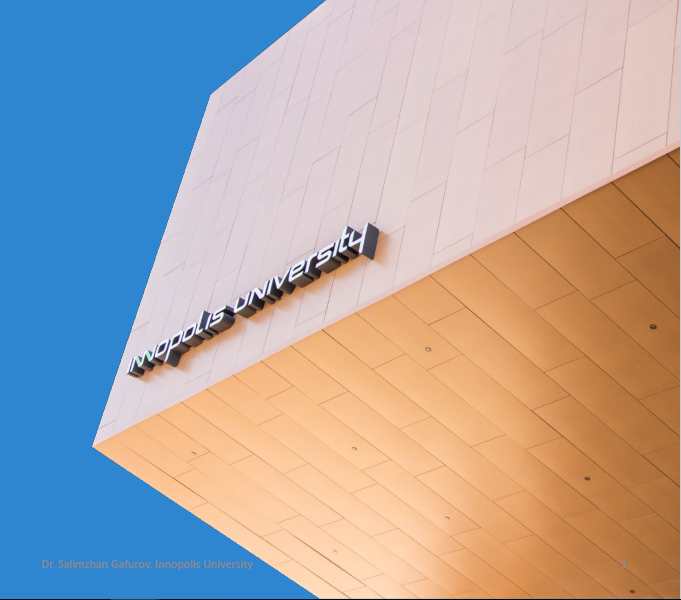
\includegraphics[width=15cm]{Innopolis_image.png}} 
\date{\today}

\begin{document}
\pagenumbering{arabic}
\setcounter{page}{1}
\setcounter{secnumdepth}{1}
	
\fontfamily{ptm}\selectfont

\maketitle

\titlelabel{\thetitle)\quad}
\titlespacing{\chapter}{0cm}{0cm}{0cm}
\titlespacing{\section}{0.2cm}{0cm}{0cm}

\textbf{NB:THE SOURCE CODE IS ATTACHED TO THE PRESENT FILE} 


\subsection{TASK 1: Finding the center of the object in the 3D space:}

We place a 3d object (a cube) in an appropriate way with respect to Kinect, the task is to associate depth map with RGB information in order to isolate the object

We use Kinect 2.0 to take RGB and depth images of our object: 
\begin{center}
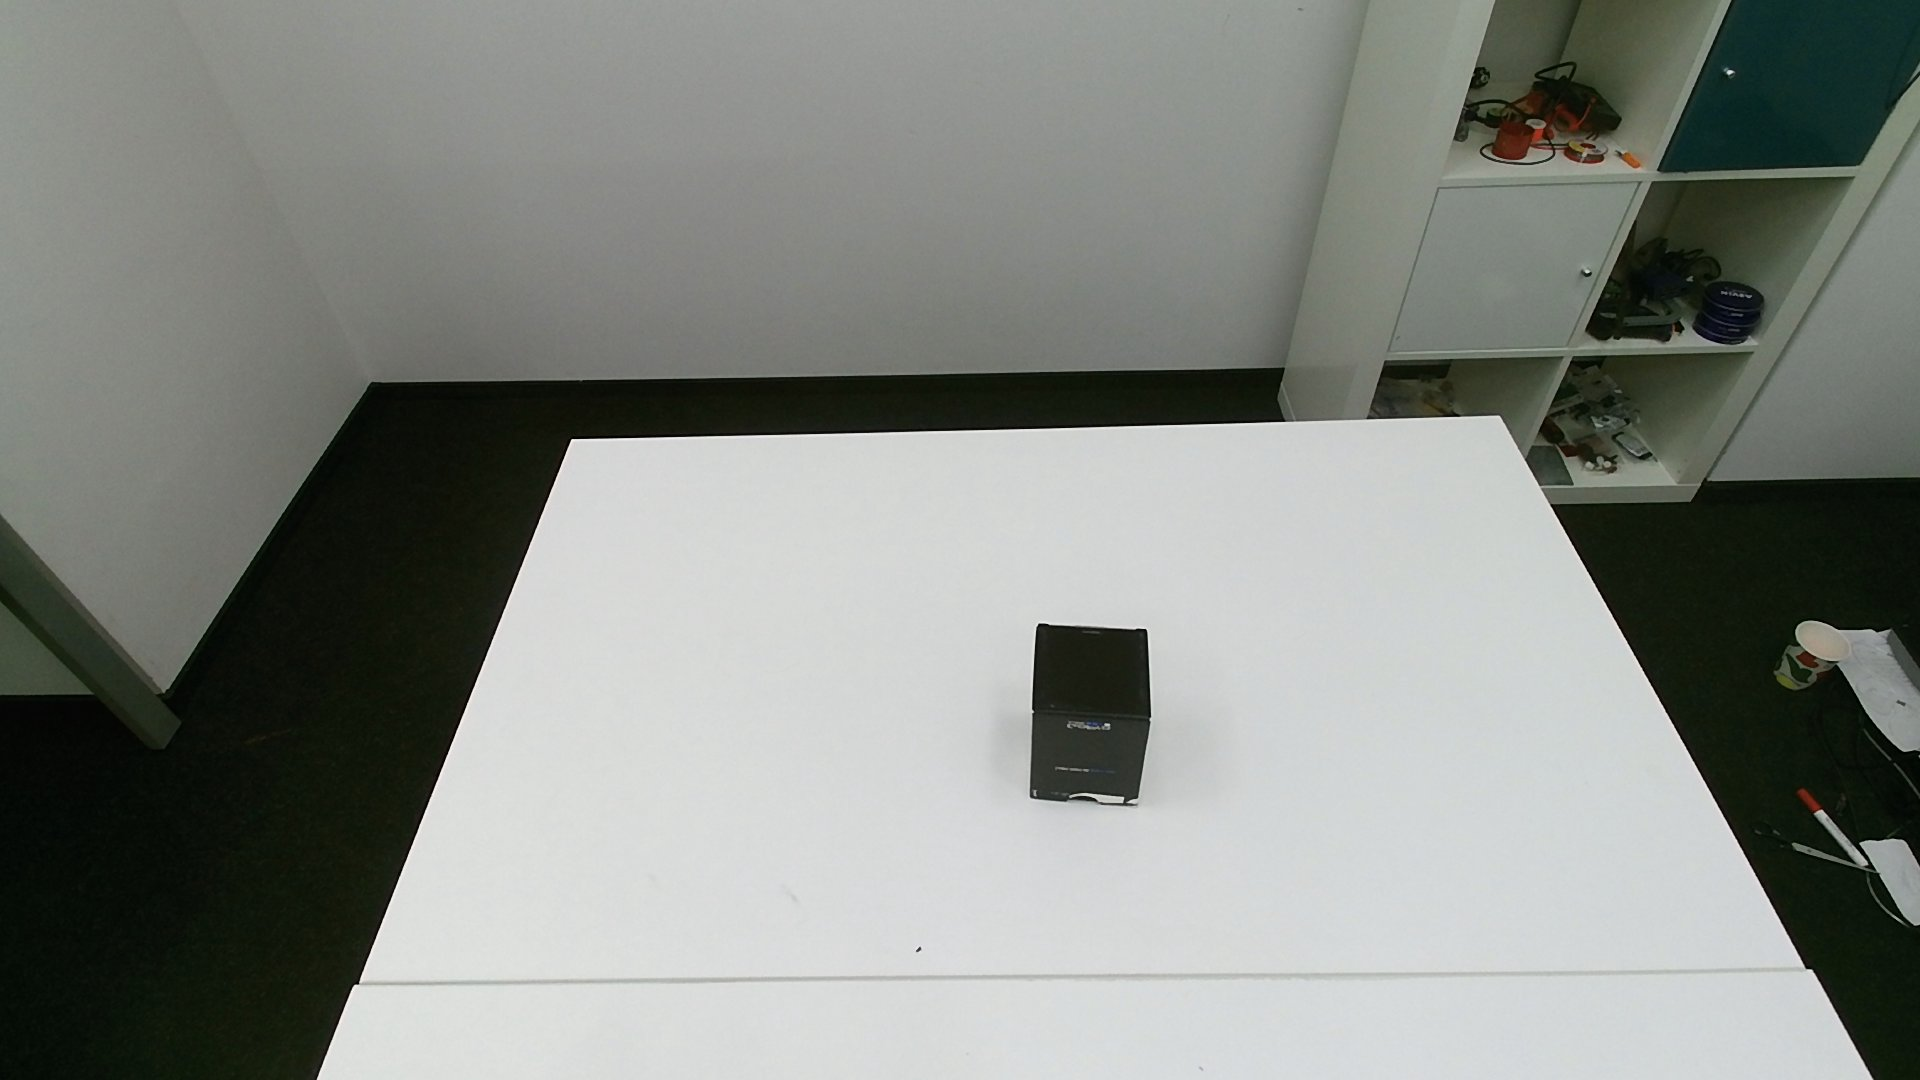
\includegraphics[width=8cm]{Capture4.jpg}
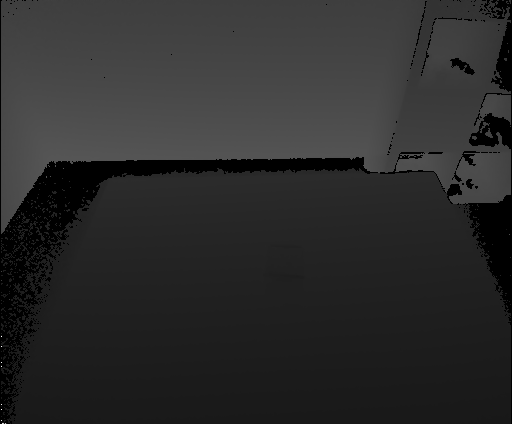
\includegraphics[width=5.5cm]{Capture5.png}
\captionof{figure}{RGB and Depth images of our 3D object}
\end{center}

We use an algorithm to extract the object and draw a rectangle around it from the RGB image and we obtain:
\begin{center}
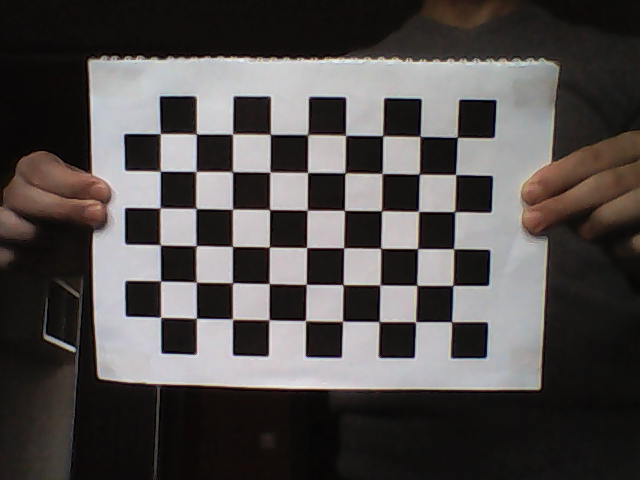
\includegraphics[width=10cm]{Capture6.png}
\captionof{figure}{Object extracted from the RGB image}
\end{center}

We calculate the center of the rectangle surrouding the object
\begin{center}
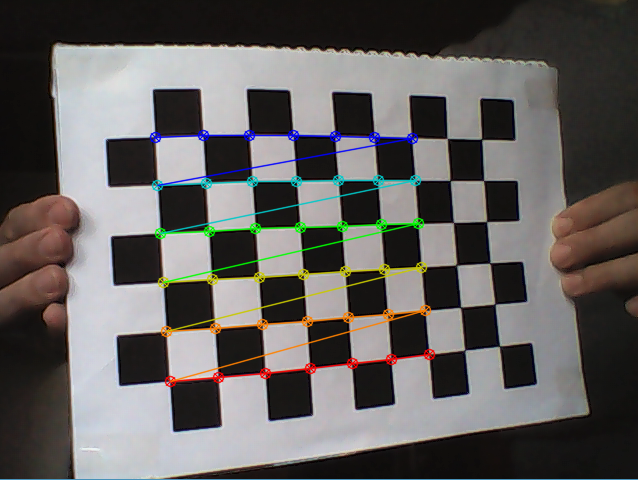
\includegraphics[width=10cm]{Capture7.png}
\captionof{figure}{Center of the object in the RGB image}
\end{center}

The center point in RGB image is  $C_{RGB}= [714\quad 1090]$

From that point knowing the resolutions of the RGB and depth images, we can compute the coordinates of the center point in the depth image by a simple rule of three:

pointDepth= pointRGB *resolutionDepth/resolutionRBG 

And we find the center point in depth image:  $C_{depth}= [280\quad 290]$ which correspond to the level of gray LG= 32 
\begin{center}
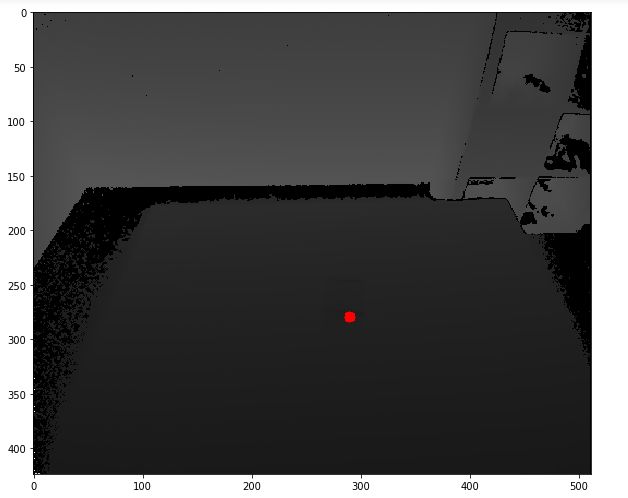
\includegraphics[width=8cm]{Capture8.png}
\captionof{figure}{Center of the object in the depth image}
\end{center}

To obtain the distance corresponding to the this level of gray, we have to calibrate our measurements, for that we place an object at a know distance d and we measure the corresponding value of level of gray 

for d = 60cm, we find LG=15, So we can say that each level of gray correspond to a distance of 4cm

Finally we can extract the distance of the object with respect to the kinect 
$$z_{object}=32\times 4 = 128 cm$$

The video of our experimentation can be viewed in this link \href{https://drive.google.com/file/d/1OEsvAl61pb7uJY_YpaSLdzBjhnByoN81/view}{Video Experiment}  


\subsection{TASK 2: Multidimensional KALMAN Filter:}
We want to estimate our trajectory while running for $100m$ with a constant speed using KALMAM Filter, for this we collected dataset containing GPS data( altitude, latitude, longitude) and linear acceleration along the three axis  

First we need to convert the GPS data into Cartesian coordinates x, y, z:
for that we use the following formulas:

\begin{eqnarray}
\left\{\begin{array}{c} 
 x =   R \ cos (lat)  \cos (long) \\ 
 y = R \ sin (lat)  \sin (long)\\  
 z = R \sin (lat)  \\ 
 \end{array} \right.
\end{eqnarray}

Where R is the radius of the earth

\begin{center}
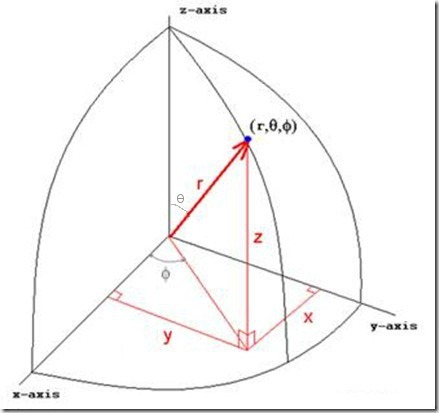
\includegraphics[width=5cm]{Capture1.jpg}
\captionof{figure}{x, y, z as functions of latitude and longitude}
\end{center}

After that since we are only interested in the variations of the position from our starting point, we need to subtract our  data position from the initial position in all axis x, y and z

We know the general equation of motion of any particle   
$$ x= x(t_0) + v(t) t + \dfrac12 a(t) t^2 $$

Or in discrete form for the three axis:
$$ x(k)= x(k-1) + v_x(k) \Delta t + \dfrac12 a_x(k) \Delta t^{2} $$
$$ y(k)= y(k-1) + v_y(k) \Delta t + \dfrac12 a_y(k) \Delta t^{2} $$
$$ z(k)= z(k-1) + v_z(k) \Delta t + \dfrac12 a_z(k) \Delta t^{2} $$

If we choose the state vector 
$$\overline{x}=\left(\begin{array}{c}
x\\
y\\
z\\
\dot{x}\\
\dot{y}\\
\dot{z}\\
\end{array}\right)$$
 
We can rewrite the equations above in the matrix form:
$$\left\{\begin{array}{c} \widehat{x_{k}} = A \widehat{x_{k-1}} +  B U_{k}  \\ y_k = C \widehat{x_{k}} \end{array}\right.$$

With :
$$ A= \left[\begin{array}{cccccc}
1& 0& 0& \Delta t & 0& 0\\ 0& 1& 0& 0& \Delta t& 0\\ 0& 0& 1& 0& 0& \Delta t\\ 0& 0& 0& 1& 0& 0\\ 0& 0& 0& 0& 1& 0\\ 0& 0& 0& 0& 0& 1 \end{array} \right]
 B= \left[\begin{array}{ccc}
0.5 \Delta t^{2}& 0& 0\\ 0& 0.5 \Delta t ^{2}& 0\\ 0& 0& 0.5\Delta t^{2}\\ \Delta& 0& 0\\ 0& \Delta t& 0 \\0& 0& \Delta t
 \end{array} \right]$$

$$ C= \left[\begin{array}{cccccc}
 1& 0& 0& 0& 0& 0\\0& 1& 0& 0& 0& 0\\0& 0& 1& 0& 0& 0
 \end{array} \right]$$

Now we can apply the general formulas of tha multidimensional KALMAN Filter:
\begin{center}
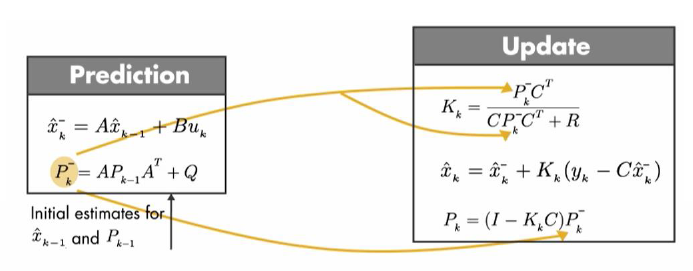
\includegraphics[width=12cm]{Capture2.png}
\captionof{figure}{Optimal state estimator}
\end{center}

The covariance matrix for our noise measurement R is set to be diagonal (the coordinates noises are independant from each other) and has the respective variances of each coordinate measurement in each diagonal element
The covariance matrix for our model Q on the other hand is set initially as an the identity matrix multiplied by a constant 
$$R= \left[ \begin{array}{ccc}
 \sigma_x^{2}& 0 & 0 \\0 & \sigma_y^{2} & 0 \\ 0& 0 & \sigma_z^{2} \end{array}\right] 
\quad Q= c^{te} \times \left[ \begin{array}{cccccc}
 1& 0 & 0& 0& 0& 0 \\0& 1 & 0& 0& 0& 0 \\0& 0 & 1& 0& 0& 0 \\0& 0 & 0& 1& 0& 0\\ 0& 0 & 0& 0& 1& 0\\0& 0 & 0& 0& 0& 1 \end{array}\right]$$

The following shows the code for computing KALMAN Filter algorithm which takes as arguments the linear accelerations, the GPS data and the time intervals:
\begin{verbatim}
def kalman(acc, z, time):
    R=np.array([[np.std(z[:, 0])**2, 0, 0], [0, np.std(z[:, 1])**2, 0], 
    [0, 0, np.std(z[:, 2])**2]])
    Q=0.05*np.identity(6)        
    x=np.zeros([z.shape[0], 6])
    P=np.identity(6)
    
    for k in range(1, z.shape[0]):
        delta=time[k]-time[k-1]        
        A= np.array([[1, 0, 0, delta, 0, 0], [0, 1, 0, 0, delta, 0], [0, 0, 1, 0, 0, delta], 
        [0, 0, 0, 1, 0, 0],[0, 0, 0, 0, 1, 0], [0, 0, 0, 0, 0, 1]])
        B= np.array([[0.5*delta**2, 0, 0], [0, 0.5*delta**2, 0], [0, 0, 0.5*delta**2], 
        [delta, 0, 0],[0, delta, 0], [0, 0, delta]])
        H= np.array([[1, 0, 0, 0, 0, 0], [0, 1, 0, 0, 0, 0], [0, 0, 1, 0, 0, 0]])
        
        x[k, :]=np.dot(A, x[k-1, :]) + np.dot(B, acc[k, :])
        P=np.dot(A, np.dot(P, A.T)) +Q                
        K= P.dot( H.T.dot(inv(H.dot(P.dot(H.T)) + R)))        
        x[k, :]= x[k, :] + K.dot(z[k, :] - H.dot(x[k, :]))        
        P=(np.identity(6)-K.dot(H)).dot(P)        
    return x\end{verbatim}

After Applying KALMANN Filter to our data we obtain the following plot of the y-coordinate with respect to x-coordinate:
\begin{center}
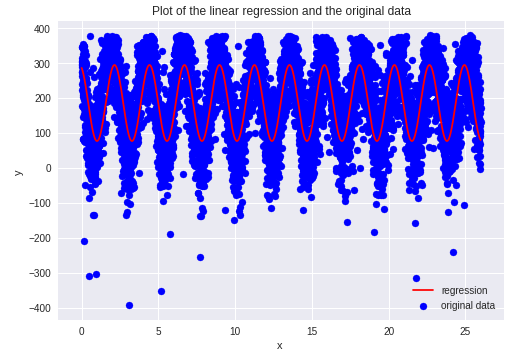
\includegraphics[width=8cm]{Capture3.png}
\captionof{figure}{Estimated trajectory}
\end{center}


\end{document}	
